\section{Sequential Datasets}
\label{sec}

There are a number of two-dimensional \ac{NMR} experiments in which the
variation of a parameter in the pulse sequence leads to the generation of
\acp{FID} of the same form except for an attenuation in their amplitudes. These
include experiments for the determination of translational diffusion rates and
relaxation properties such as $T_1$, $T_2$, and $T_{1\rho}$. Estimation of such
datasets using nonlinear programming is attractive as after the first \ac{FID}
has been estimated without \textit{a priori} information, subsequent \acp{FID}
can be estimated using the previous result as an initial guess. On top of this,
only the amplitudes of each increment need to be optimised, as the phases,
frequencies and damping factors will be unperturbed across increments.

In this chapter, a generalised approach to analysing such datasets using the
estimation procedure presented in Chapter \ref{chap:theory} is presented.

\subsection{Methodology}

\subsubsection{Outline of the problem}
There are numerous experiments in which the pulse sequence is repeated over
multiple values of a certain parameter $\symbf{v} \in \mathbb{R}^I$. Examples
of this are various relaxation experiments (Section
\ref{sec:relaxation_experiments}) in which this parameter is effectively the
amount of time relaxation is allowed to occur, and diffusion experiments
(Section \ref{sec:diffusion_experiments}) in which it is the strength of the
diffusion-encoding \acp{PFG}. These experiments lead to an FID $\symbf{Y} \in
\mathbb{C}^{I \times N}$ in which the value of the experimental parameter
attenuates the amplitudes of the contributing resonances:
\begin{equation}
    Y[i, n] = \sum_{m=1}^M a_m^{(i)} \exp\left(\iu \phi_m\right)
        \exp\left(\left(2 \pi \iu f_m - \eta_m \right) n \Dt\right).
\end{equation}
The variation of the amplitudes of all resonances is described by the parameter
vector $\symbf{p} \in \mathbb{R}^{2M}$:
\begin{equation}
    \symbf{p} = \left[
        \zeta_1, \psi_1, \zeta_2, \psi_2, \cdots, \zeta_M, \psi_M
    \right]^{\mathrm{T}}.
\end{equation}
$\symbf{\zeta} = \lbrace\zeta_1, \cdots, \zeta_M\rbrace$ are a set of scaling
parameters, one per oscillator, that are not typically of
interest, but that are necessary for extracting  $\symbf{\psi} = \lbrace
\psi_1, \cdots, \psi_M \rbrace$, the of set parameters of interest (relaxation
rates, diffusion rates, etc. associated with each oscillator). The amplitudes
vary from increment to increment as a result of some function $\mathcal{A}$,
whose form varies across different types of experiments (see Table
\ref{tab:seq_equations}). In general:
\begin{equation}
    a^{(i)}_m = a_m(v_i, \zeta_m, \psi_m) = \zeta_m \mathcal{A}\left(v_i, \psi_m \right)
\end{equation}

\begin{table}
    \begin{center}
        \begin{tabular}{ccccccc}
            \hline
            Experiment &
            $v$ &
            $\zeta$ &
            $\psi$ &
            $\mathcal{A}(v, \psi)$ &
            $\frac{\partial \mathcal{A}(v, \psi)}{\partial \psi}$ &
            $\frac{\partial^2 \mathcal{A}(v, \psi)}{\partial \psi^2}$ \\ \hline
            Inversion Recovery &
            $\tau$ &
            $a_{\infty}$ &
            $T_1$ &
            $\left(1 - 2 \exp \left(-\frac{\tau}{T_{1}}\right)\right)$ &
            $-\frac{2 \tau}{T_1^2} \exp\left(-\frac{\tau}{T_1}\right)$ &
            $\frac{2 \tau}{T_1^3} \exp\left(-\frac{\tau}{T_1}\right)\left(2 - \frac{\tau}{T_1}\right)$\\
            CPMG &
            $n_{\textrm{cycles}}$ &
            $a_0$ &
            $T_2$ &
            ? &
            ? &
            ? \\
            Diffusion &
            $g$ &
            $a_0$ &
            $D$ &
            $\exp\left(-c g^2 D\right)$ &
            $-c g^2 \exp\left(-c g^2 D\right)$ &
            $c^2 g^4 \exp\left(-c g^2 D\right)$ \\
            \hline
       \end{tabular}
       \caption{
           The various functional forms of $\mathcal{A}$ according to the
           different sequential NMR experiments considered in this thesis.
           $\mathcal{A}$ describes how the amplitude of a resonance is affected
           by the experimental parameter $v$.
       }
       \label{tab:seq_equations}
    \end{center}
\end{table}

Determination of $\psi_m$, the parameter of interest for a given oscillator can be achieved by nonlinear programming, via optimisation of the fidelity
\begin{subequations}
    \begin{gather}
        \mathcal{F}\left(\zeta_m, \psi_m | \symbf{v}\right) =
            \left \lVert \symbf{a}_m - \zeta_m \mathcal{A} \left(\symbf{v},
            \psi_m\right) \right\rVert_2^2,\\
        \symbf{a} = \left[a_m^{(1)}, a_m^{(2)}, \cdots,
            a_m^{(I)}\right]^{\mathrm{T}}.
    \end{gather}
\end{subequations}

Derivatives:
\begin{subequations}
    \begin{gather}
        \frac{\partial \zeta_m \mathcal{A} \left(v_i, \psi_m\right)}
            {\partial \zeta_m} =
            \mathcal{A}\left(v_i, \psi_m\right) \\
        \frac{\partial \zeta_m \mathcal{A} \left(v_i, \psi_m\right)}
            {\partial \psi_m} =
            \zeta_m \frac{\partial\mathcal{A}\left(v_i, \psi_m\right)}{\partial \psi_m}\\
        \frac{\partial^2 \zeta_m \mathcal{A} \left(v_i, \psi_m\right)}
            {\partial \zeta_m^2} = 0\\
        \frac{\partial^2 \zeta_m \mathcal{A} \left(v_i, \psi_m\right)}
            {\partial \psi_m \partial \zeta_m} =
            \frac{\partial^2 \zeta_m \mathcal{A} \left(v_i, \psi_m\right)}
            {\partial \zeta_m \partial \psi_m} =
            \frac{\partial\mathcal{A}\left(v_i, \psi_m\right)}{\partial \psi_m}\\
        \frac{\partial^2 \zeta_m \mathcal{A} \left(v_i, \psi_m\right)}
            {\partial \psi_m^2} =
            \zeta_m \frac{\partial^2 \mathcal{A}\left(v_i, \psi_m\right)}{\partial \psi_m^2}\\
    \end{gather}
\end{subequations}

It therefore is necessary to determine the amplitudes of a given oscillator for a given increment, which is desribed in the next section

\subsubsection{Determining amplitudes}


\subsection{Relaxation experiments}
\label{sec:relaxation_experiments}

Integrals of peaks modelled with two parameters $\symbf{\theta} \in \mathbb{R}^2$:
\begin{subequations}
   \begin{gather}
        \theta_1 = I_{\infty} = \lim_{\tau \rightarrow \infty} x\\
        \theta_2 = T_1
   \end{gather}
\end{subequations}

\begin{equation}
    \symbf{I}\left(\symbf{\theta}, \symbf{\tau}\right) =
        I_{\infty} \left[ 1 - 2 \exp\left( -\frac{\symbf{\tau}}{T_1}\right) \right],
\end{equation}

Fitting this function is achieved by minimising L2-norm (reference it in
previous discussion, and refer to grad and Hessian). The first and second
derivatives of the model, required to construct the grad and Hess are
\begin{subequations}
    \begin{gather}
        \frac{\partial I}{\partial I_{\infty}} =
            1 - 2 \exp \left( -\frac{\tau}{T_1} \right)\\
        \frac{\partial I}{\partial T_1} =
        -\frac{2 I_{\infty} \tau}{T_1^2} \exp\left( -\frac{\tau}{T_1} \right)\\
        \frac{\partial^2 I}{\partial I_{\infty}^2} = 0\\
        \frac{\partial^2 I}{\partial I_{\infty} \partial T_1} =
            \frac{\partial^2 I}{\partial T_1 \partial I_{\infty}} =
            -\frac{2 \tau}{T_1^2} \exp\left(- \frac{\tau}{T_1} \right)\\
        \frac{\partial^2 I}{\partial T_1^2} =
            \frac{2 I_{\infty} \tau}{T_1^3} \exp\left(- \frac{\tau}{T_1} \right)
            \left(2 - \frac{\tau}{T_1}\right)
    \end{gather}
\end{subequations}

\subsection{Diffusion experiments}
\label{sec:diffusion_experiments}

Along with their widespread use in dephasing undesired coherences in a pulse
sequence, the use of \acp{PFG} is central to determining translational
diffusion properties of species with NMR. The first showcase for extracting
translational diffusion coefficients came from Stejskal and Tanner in 1965, in
which they introduced the \ac{PGSE} pulse sequence\cite{Stejskal1965} (Figure
\ref{fig:diffusion_sequences}.a).

The \ac{PGSE} sequence consists of a conventional spin-echo ($\ang{90}
\xrightarrow{\tau} \ang{180} \xrightarrow{\tau} \text{acquire}$), with
\acp{PFG} applied after each of the \ac{RF} pulses.
As a simple overview of how the pulse sequence works, consider a single spin on
resonance with the transmitter (i.e. its rotating frame frequency is zero) in a
sample tube at position $z$ along the axis collinear with the main field.
After the \ang{90} pulse, the magnetisation will be $-M_y$.
During the first \ac{PFG}, the spin's resonance frequency will become
$\omega_{\text{PFG}} = -\gamma g z$, where $g$ is the strength of the \ac{PFG}.
Assuming the gradient is applied for a time $\delta$, the spin will
precess by an angle of  $\alpha = -\gamma g z \delta$. After the \ang{180}
pulse, the spin's magnetisation is as follows:
\[
    -M_y
    \xrightarrow{\text{PFG}} -M_y \cos(\alpha) + M_x \sin(\alpha)
    \xrightarrow{\ang{180}_y} -M_y \cos(\alpha) - M_x \sin(\alpha).
\]
Supposing that the spin has moved to a new position $z + \Delta_z$
between the end of the first gradient and the beginning of the second,
application of the second gradient causes precession by the angle
$\beta = -\gamma g (z + \Delta_z) \delta$:
\begin{equation*}
   \begin{split}
        \xrightarrow{\text{PFG}}
            &-M_y \cos(\alpha)\cos(\beta) +
            M_x \cos(\alpha)\sin(\beta) -
            M_x \sin(\alpha)\cos(\beta) -
            M_y \sin(\alpha)\sin(\beta)\\
        &= -M_y \cos(\gamma g \delta \Delta_z) -
           M_x \sin(\gamma g \delta \Delta_z),
   \end{split}
\end{equation*}
In the scenario that the spin has not translated in the $z$-direction between
\acp{PFG} ($\Delta_z = 0$), the net effect of the pulse sequence is nothing
(except for a loss of signal amplitude through $T_2$ relaxation). However, if
translation does occur, the signal phase is adjusted, as a function of the
extent of translation $\Delta_z$. The gradients have effectively been employed
to encode the change in position of the spin after a known amount of time.
Extending this idea to a system of many identical spins, which will translate
by different extents between the \acp{PFG}, individual spin contributions to
the bulk magnetisation will become dephased, leading to an attenuation of the
amplitude of the resulting FID.

\begin{figure}
   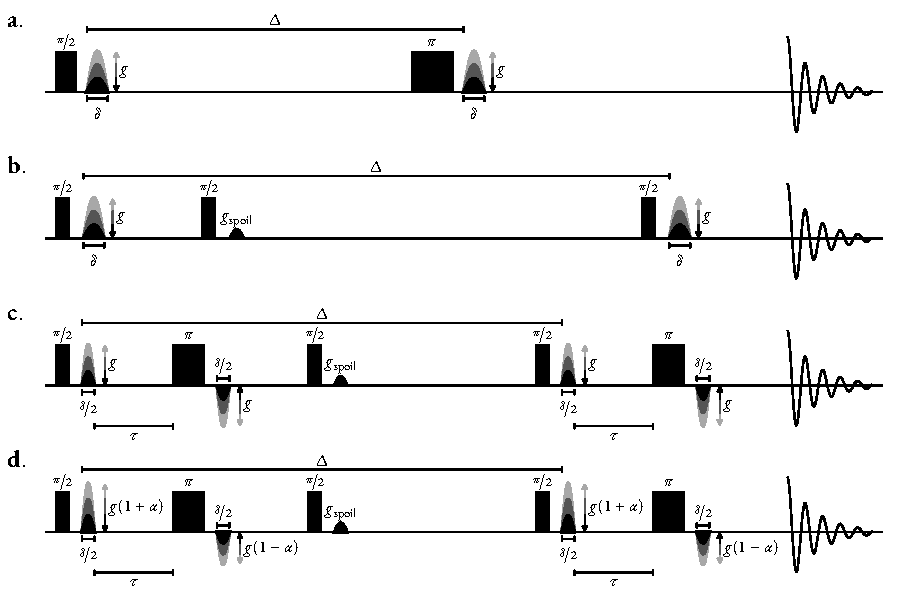
\includegraphics{diffusion_sequences/diffusion_sequences.pdf}
   \caption[
       Pulse sequences used for the determination of translational diffusion constants.
   ]{
       Pulse sequences used for the determination of translational diffusion constants.
       \textbf{a.} \acs{PGSE},
       \textbf{b.} \acs{PGSTE},
       \textbf{c.} \acs{PGSTEBP},
       \textbf{d.} One-shot DOSY.
       \ac{RF} pulses are denoted by solid rectangles. Diffusion-encoding
       gradients are denoted by sine-bell shapes with varying shades,
       indicating that the intensity is incremented to create a \ac{2D}
       dataset. Spoiler gradients are denoted by solid black sine-bell shapes.
   }
   \label{fig:diffusion_sequences}
\end{figure}

Through consideration of the Bloch-Torrey equations\cite{Torrey1956}, which
extend the classic Bloch equations to account for the effects of diffusion on
magnetisation, Stejskal and Tanner were able to derive the following equation
for the variation of the amplitude of a resonance as a function of gradient
strength, known widely as the Stejskal-Tanner equation:
\begin{equation}
    a(g) = a_0 \exp \left(- \gamma^2 \delta^2 g^2 D \left(\Delta -
    \frac{\delta}{3}\right)\right),
    \label{eq:stejskal_tanner}
\end{equation}
where
$a_0 = \lim_{g \rightarrow 0} a$,
$\gamma$ is the gyromagnetic ratio of the target nucleus
(\unit{\mega\hertz\per\tesla}),
$g$ is the gradient strength (\unit{\tesla\per\meter})\footnote{
    Gradient strengths are often expressed in units of
    \unit{\gauss\per\centi\meter}, which is equivalent to
    \qty[print-unity-mantissa = false]{e-2}{\tesla\per\meter}.
},
$\delta$ is the duration of the \acp{PFG} (\unit{\second}),
$\Delta$ is the delay between the \acp{PFG}, often known as the diffusion time
(\unit{\second}),
and $D$ is the translation diffusion constant of the species giving rise to the
resonance (\unit{\meter\square\per\second}).
While Equation \ref{eq:stejskal_tanner} is widely stated in the literature, it
is only technically applicable to the scenario in which the \ac{PGSE} sequence
is used (or any other \emph{monopolar} sequence, \emph{vide infra}), and
rectangular \acp{PFG} are applied
\footnote{
    Rectangular \acp{PFG} (i.e. those in which there is an infinitesimal time
    to rise to full strength, and to fall back to zero) are in fact
    impossible to achieve as they would require gradient coils with zero
    inductance.
}.

Tanner introduced a variant on the original \ac{PGSE} experiment called
\ac{PGSTE}\cite{Tanner1970} (Figure \ref{fig:diffusion_sequences}.b). Instead
of the diffusion period including a
\ang{180} pulse, \ac{PGSTE} has two \ang{90} pulses, with the first being
applied shortly after the initial \ac{PFG}, and the second being applied just
before the second \ac{PFG}. The key difference between this and the \ac{PGSE}
experiment is that relaxation of the signal during the diffusion time is
dictated by longitudinal relaxation ($T_1$), rather than transverse relaxation
($T_2$). \ac{PGSTE} is therefore favoured in scenarios where $T_1 \ll T_2$, as
improved sensitivity will be achieved in the resulting \ac{FID}.


Both \ac{PGSE} and \ac{PGSTE} employ \emph{monopolar} \acp{PFG} for diffusion
encoding, in the sense that they are both polarised in a
single direction. Experiments also exist which employ
\emph{bipolar} gradient elements\cite{Cotts1989,Wu1995}, which consist of a
\ac{PFG}, followed by a \ang{180} pulse, and then a second \ac{PFG} with the
opposite polarity to the first. A well-known example is the \ac{PGSTEBP}
experiment (Figure \ref{fig:diffusion_sequences}.c). Bipolar gradient are
useful in circumstances where it is important to purge the effects of static
gradients in the sample, caused by field inhomogeneities. Morris and coworkers
have also developed the One-shot DOSY experiment\cite{Pelta2002} (Figure
\ref{fig:diffusion_sequences}.d), which requires a single transient per
gradient strength (i.e. there is no requirement for a phase-cycling scheme).
This is achieved through the use of bipolar gradients which comprise
asymmetrical \acp{PFG} with relative powers $1 + \alpha : 1 - \alpha$ for some
$\alpha > 0$
\footnote{
    $\alpha$ is typically set to be considerably less that $1$, commonly $0.2$.
}.
\note{Cite some review articles (Johnson, Morris 2009)}

It is virtually always the case that the amplitudes of each resonance in the
\ac{FID} abide by the following general form of the Stejskal-Tanner equation:
\begin{equation}
    a(g) = a_0 \exp\left(- c g^2 D\right)
\end{equation}
for some constant $c$ (\unit{\tesla\per\second\squared}).
It is important to note that functional form of $c$ is highly variable
dependent on the type of experiment used, and its value if affected by the
shape of the diffusion-encoding \acp{PFG}. A consideration of the Bloch-Torrey
equation for a given experiment is necessary, with an extensive overview
provided by Sinnaeve for most diffusion NMR experiments\cite{Sinnaeve2012}. In
general, $c$ is as follows:
\begin{equation}
    c = \gamma^2 \delta^2 \sigma^2 \Delta^{\prime}.
    \label{eq:stejskal_tanner_generic}
\end{equation}
$\sigma$ is the \emph{shape factor} of the \acp{PFG} (\emph{vide infra}), and
$\Delta^{\prime}$ is the effective time that diffusion is allowed to occur.
Examples of the value of $\Delta^{\prime}$ include:
\begin{subequations}
    \begin{alignat}{2}
        & \text{Monopolar gradients (\ac{PGSE}, \ac{PGSTE})} \quad && \Delta + 2 \left(\kappa - \lambda\right) \delta,
        \label{eq:monopolar}\\
        & \text{Bipolar gradients (\ac{PGSTEBP})} \quad && \Delta + \frac{\left(2 \kappa - 2 \lambda
            - 1\right)\delta}{4} - \frac{\tau}{2},\\
        & \text{One-shot}
            \quad && \Delta + \frac{\left(\kappa - \lambda\right)
            \left(\alpha^2 + 1\right) \delta}{2} +
            \frac{\left(\delta + 2 \tau\right)\left(\alpha^2 - 1\right)}{4}.
    \end{alignat}
\end{subequations}
$\tau$ is the delay between the initial \ac{PFG} and the \ang{180} pulse in
experiments with bipolar gradients.
The factors $\sigma$,  $\lambda$, and $\kappa$ are related to the shape
function $s(\epsilon) : \epsilon \in [0, 1]$ of the \ac{PFG}, which describes
the variation in the intensity of the gradient as a function of its progression.
For a rectangular gradient, $s(\epsilon) = 1 \forall \epsilon$, whereas for a
sine-bell gradient, $s(\epsilon) = \sin(\pi \epsilon)$. The cumulative
distribution of the shape function is given by:
\begin{equation}
    S(\epsilon) = \int_0^{\epsilon} s\left(\epsilon^{\prime}\right)
            \mathrm{d} \epsilon^{\prime} \quad \forall \epsilon \in [0, 1].
\end{equation}
The corresponding definition of $S$ for the case of a gradient made of discrete
steps with shape function $\symbf{s} \in \mathbb{R}^{N_g}$ is
\begin{equation}
    S\left[n\right] =
        \frac{1}{n} \sum_{i = 0}^{n} s\left[i\right] \quad
        \forall n \in \left\lbrace 0, \cdots, N_g - 1\right\rbrace,
\end{equation}
where $N_g$ is the number of points the gradient comprises. The three factors
are given by
\begin{subequations}
    \begin{gather}
        \sigma = S(1),\\
        \lambda = \frac{1}{\sigma} \int_0^1 S(\epsilon) \mathrm{d} \epsilon,\\
        \kappa = \frac{1}{\sigma^2} \int_0^1 S^2(\epsilon) \mathrm{d} \epsilon,
    \end{gather}
\end{subequations}
with their discrete counterparts being
\begin{subequations}
    \begin{gather}
        \sigma = S\left[N_g - 1\right] \\
        \lambda = \frac{1}{\sigma N_g} \sum_{n = 0}^{N_g - 1} S\left[n\right]
            = \frac{1}{\sigma N_g} \sum_{n = 0}^{N_g - 1}
            \frac{1}{n} \sum_{i=0}^{n} s\left[i\right]\\
        \kappa = \frac{1}{\sigma^2 N_g} \sum_{n = 0}^{N_g - 1} S^2\left[n\right]
            = \frac{1}{\sigma^2 N_g} \sum_{n = 0}^{N_g - 1}
            \frac{1}{n^2} \left(\sum_{i=0}^{n} s\left[i\right]\right)^2
    \end{gather}
\end{subequations}
For \acp{PFG} with a symmetrical shape, $\lambda = \nicefrac{1}{2}$. $\kappa$
is typically equal to or close to $\nicefrac{1}{3}$. It can now be seen that
Equation \ref{eq:stejskal_tanner} comes from plugging Equation
\ref{eq:monopolar} into Equation \ref{eq:stejskal_tanner_generic}, with $\sigma
= 1$,  $\lambda = \nicefrac{1}{2}$, and  $\kappa = \frac{1}{3}$. In many
situations,  $\Delta$ dominates in the expression of $\Delta^{\prime}$, and so
ensuring the correct form of $c$ could be seen as excessive. However,
especially when  $\Delta$ is not orders of magnitude greater than $\delta$, the
exact form of $\Delta^{\prime}$ used in Equation
\ref{eq:stejskal_tanner_generic} will be extremely important for accurate
measurements of $D$.

The necessary first and second derivatives required to estimate the translational diffusion constant using the \ac{Trust NCG} algorithm are:
\begin{subequations}
   \begin{gather}
       \frac{\partial a}{\partial a_0} = \exp\left(-c g^2 D\right) \\
       \frac{\partial a}{\partial D} = -a_0 c g^2 \exp\left(-c g^2 D\right) \\
       \frac{\partial^2 a}{\partial a_0^2} = 0\\
       \frac{\partial^2 a}{\partial a_0 \partial D} =
           \frac{\partial^2 a}{\partial D \partial a_0} =
           -c g^2 \exp\left(-c g^2 D\right) \\
       \frac{\partial^ 2 a}{\partial D^2} = a_0 c^2 g^4 \exp\left(-c g^2 D\right)
   \end{gather}
\end{subequations}

\begin{equation}
    \frac{\partial^n x}{\partial D^n} = \left(-c G^2\right)^n \exp\left(-c D G^2\right)
\end{equation}

\subsection{Plotting DOSY-type results}
Spectrum $S \in \mathbb{R}^{N, I}$ is given by
\begin{subequations}
    \begin{gather}
        S = \sum_{m=1}^M \symbf{s}_m \otimes \frac{\symbf{d}}{\max\left(\symbf{d}\right)} \\
        \symbf{s}_m = \FT\left\lbrace
            a^{(1)}_m \exp\left(\iu \phi_m\right) \exp\left(\left(2 \pi \iu f_m - \eta_m\right) \symbf{n} \Dt\right)
        \right\rbrace \\
        \symbf{d}  = \exp\left(
            -\frac{\left(\symbf{y} - \theta_2\right)^2}
            {2 \sigma_2^2}
        \right)
    \end{gather}
\end{subequations}
